\documentclass{sig-alternate}
\usepackage[utf8]{inputenc}
\usepackage{blindtext, graphicx, pgfplots}
\usepackage[backend=biber,sorting=none]{biblatex}
\addbibresource{references.bib}
\setlength{\paperheight}{11in}
\usepackage{microtype}
\usepackage{hyperref}
\usepackage[all]{hypcap}
\pgfplotsset{compat=1.10,
    /pgfplots/ybar legend/.style={
    /pgfplots/legend image code/.code={%
       \draw[##1,/tikz/.cd,yshift=-0.25em]
        (0cm,0cm) rectangle (3pt,0.8em);},
   },
}
\graphicspath{{images/}}

\begin{document}

\setcopyright{rightsretained}

\title{B-09/8: Performance and Availability of Galera Cluster with MariaDB on Amazon Cloud – a case study}

\include{pubinfo}

\maketitle
\begin{abstract}
Traditional approaches to database replication (like MySQL replication) are considered server-centric (master / slave), as they basically stream data from one server to another. Server-centric approaches bring with them certain problematic situations like the consequences of a node-crash, the not-knowing of which node has a specific dataset or having to find ways to backup the cluster. This paper offers Galera Cluster as a solution to these problems, as it is data-centric and offers more security and power. We explore related work in the area of database replication and furthermore replication using a Galera Cluster. We look into the performance and availability of a Galera Cluster, while using MariaDB (a community-developed fork of the MySQL relational DBMS) on Amazon Cloud. In that effort we create one dataset and firstly monitor the throughput and response time of one node. Afterwards we gradually add Galera replicas and explore how the response time of the cluster changes and how many requests we can process, as we increase the number of replicas and the number of clients.
\end{abstract}

\keywords{Galera Cluster, MariaDB, Database replication, High availability, Performance, Amazon Cloud}

\section{Introduction}
\subsection{State of the art}
Traditional approaches to database replication (like MySQL replication) are considered server-centric (master / slave), as they basically stream data from one server to another. Server-centric approaches bring with them certain problematic situations like the consequences of a node-crash, the not-knowing of which node has a specific dataset or having to find ways to backup the cluster.

\bigskip

\subsection{Problem}
The problems are that on the one hand slave DBs are not updated in real-time, which can lead to a loss of data and on the other hand they are expensive and time-consuming to manage. Furthermore the inability to scale out when needed poses a threat to monetizing on business opportunities.

\subsection{Proposed solution to problem}
Galera Cluster is a synchronous, multi-master-cluster that replaces MySQL binlog/replication. An application working through a Galera Cluster can read and write from any DB-node and experiences no slave lag or integrity issues. Galera Cluster furthermore offers features like synchronous replication, active-active multi-master topology and automatic node provisioning.

\subsection{Related work}
Database Multi-master replication is used in a Learning Assistance System \cite{gautam2016multi}. Replication is the key to improve availability but problems are to guarantee consistency, availability and partition tolerance.
Active replication means to process the same request at every replica, whereas with passive replication each single request is processed on a single replica and then its state is transferred to the other replicas.
Multi-master replication is a method of DB replication, which allows data to be stored by a group of computers, and updated by any member of the group.

In order to address those problems consistency-aware protocols are used. Active eager replication based on the optimistic approach (local replicas to interrupt for correction) is used with Galera cluster for content related to Moodle to address and to ensure local consistency for each cluster. Passive lazy replication is accomplished by a user writing queries for the cluster. It works with a dedicated algorithm. 

Pacitti et al. \cite{pacitti2003preventive} demonstrate preventive multi-master lazy replication assuring strong consistency without the constraints (expensive in terms of message overhead and response time) of eager replication. A multi-master refresher algorithm prevents conflicts by exploiting the cluster’s high speed network. Their solution achieves full node autonomy with independent black box cluster nodes.

\bigskip

\subsection{Structure of paper}
Firstly we take a deeper look at Galera Cluster and the implications of this technology, so that the context of this paper is clearer. Afterwards a Galera Cluster with a constant dataset is implemented and changes in the cluster’s throughput and response time are monitored, as more nodes are added to the cluster. We then sum up our work and the key learning points.

\section{Galera Cluster}
\subsection{Overview of Galera Cluster}

\begin{figure}[ht]
	\centering
	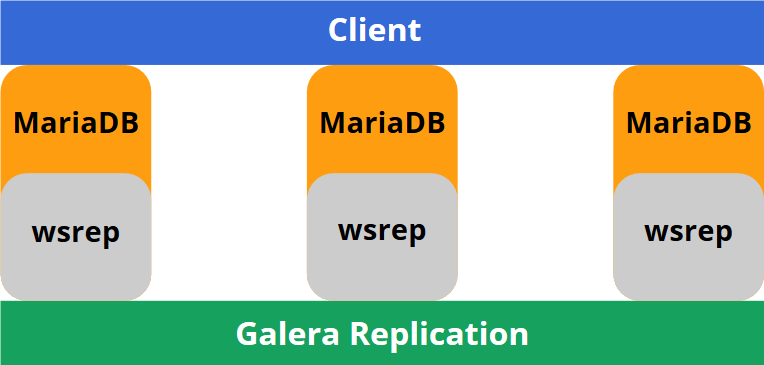
\includegraphics[width=6cm]{galera1-2.png}
	\caption{MariaDB Galera basic architecture}
	\label{fig:galera_structure}
\end{figure}

Fig \ref{fig:galera_structure} shows the basic architecture of a MariaDB Galera Cluster, where clients can on the one hand connect to any node and on the other hand have read and write access to any node. There can be several nodes with automatic node provisioning and synchronous replication. To the client the multi-master cluster looks like one big database with multiple entry points. Once a client reads or writes to a node, the transaction is processed locally up to commit time and is then replicated to the whole cluster. The load balancer, which divides the amount of incoming work between all nodes, notices the error and removes the node from the pool.

\subsection{Architecture of Galera Cluster}

Wsrep API (Write-Set Replication API) is a generic replication API for DBMS-like applications, with which Galera Cluster delivers certification-based replication. It consists of “wsrep hooks", which is the “integration with the database server engine and \texttt{dlopen()}, which makes the wsrep provider available to the wsrep hooks” \cite{wsrepapi}. Wsrep considers the database server to have a state, which refers to the contents of its database. When the database is in use and its content is changed, the state of the database is also changed and the wsrep API represents the changes as a series of atomic transactions. In a database cluster all nodes have the same state, as they continually synchronize by applying the same atomic transactions in the same order.

So when a change in the state of a server occurs, the wsrep-hooks translate the changes to the write-set, \texttt{dlopen()} make the wsrep provider functions available and the Galera Replication Plugin enables write-set replication service functionality.

To identify state changes the wsrep API uses a GTID (Global Transaction ID), which consists of State UUID (unique identifier for the state and the order of atomic transactions that were applied to it) and Ordinal Sequence Number, which is used to identify the position of the change in sequence \cite{wsrepapi}.

\subsection{Failure and Recovery}

One can differentiate between individual node failure and component failure, where individual node describes one singular node getting disconnected from the cluster, due to some unforeseen fault like a hardware crash or loss of connectivity.

A node is considered failed when the primary component can no longer see it, whereas a component is defined as multiple nodes connected to each other and the primary component of a Galera cluster is the one component that can modify the database state. The failure of a singular node has no major consequences, as the other nodes continue working and the failed node can join the cluster again, after it came back online and successfully replicated the data from the existing nodes. As a server administrator one can find out about node status, by polling the \texttt{wsrep\_local\_state} variable or using a notification command \cite{galerarecovery}.

When a major network failure happens, the Galera cluster may be split into various similar components. In this situation the cluster has to decide which component is considered as the primary component, meaning which component has the say about which state of the database is correct. For deciding on the primary component, Galera cluster firstly uses a weighted quorum method, where every node gets a weight ranging from 0 to 255 and then secondly calculates which component is considered primary \cite{galeraquorum}.

\section{Implementation}
Amazon Cloud (AWS) has been used to create a cluster of 5 nodes, each being a production-ready r4.xlarge instance optimized for database workloads \cite{awsinstances} with 4 Xeon E5-2686 v4 cores and 30 GB of DDR4 RAM. As a storage the General Purpose SSD volumes have been used, with a capacity of 500 GB and 1500 IOPS each. The seemingly unnecessary capacity was required to reach high IOPS, since Amazon provides 3 IOPS per GB for this type of storage. To minimize latency the nodes were placed in the same availability zone, in the same Virtual Private Cloud (VPC) and connected over a 10 gigabit network.

On the software side, CentOS 7.3 with the 3.10.0-514 Linux kernel has been chosen as the operating system. Volumes were mounted with the XFS journaling file system. The tested database versions were MariaDB 10.1.20 and Galera 25.3.19.

All the relevant configuration and testing commands can be found in appendix, with the goal to make the results fully reproducible.

\section{Simulation}

The performance evaluation has been done using Sysbench 0.5, specifically the OLTP Read/Write (RW) benchmark wich consists of 70\% read (\texttt{SELECT}) and 30\% write (\texttt{INSERT, UPDATE, DELETE}) operations, simulating a real-world usage. The dataset contained 1,000,000 rows in a single table totalling 300 MB. Sysbench is a well known set of benchmarks, used by the MariaDB team itself to uncover performance problems as a part of the development process \cite{mariadbsysbench}.

\begin{figure}[ht]
	\centering
	\begin{tikzpicture}[scale=0.85]
		\begin{axis}[
				y tick label style={/pgf/number format/.cd,%
					scaled y ticks = false,
					set thousands separator={},
				fixed},
				ybar,
				enlarge x limits=0.45,
				ylabel={Throughput (transactions per second)},
				symbolic x coords={Galera,Standalone},
				xtick=data,
				bar width=1.3cm,
				ymin=0,
				legend style={at={(0.765,0.25)},anchor=north},
			]
			\addplot coordinates {(Galera,18748) (Standalone,22135)};
			\addplot coordinates {(Galera,6061) (Standalone,19261)};
			\legend{non-durable, durable}
		\end{axis}
	\end{tikzpicture}
	\caption{Sysbench RW, single node durable vs non-durable}
	\label{fig:durable_nondurable}
\end{figure}

In the initial phases of testing it has been discovered that Galera suffers from an unusually significant performance loss compared to a standalone MariaDB when configured with so-called durable settings (\texttt{sync\_binlog=1, innodb\_flush\_log\_at\_trx\_commit=1}) which cause a 70\% performance loss even on a single-node Galera and just 16\% on standalone, as seen in Fig \ref{fig:durable_nondurable}. This could be a regression in the latest version and is currently being investigated by MariaDB upon our bug report. Fortunately, durable settings are not required for data consistency with Galera, because data loss would only occur if all nodes would lose power at the same time. Considering this, the tests were performed with non-durable settings.

\subsection{Throughput}

When measuring the peak sustainable throughput (transactions per second), we have firstly performed a test with a constant number of clients (128) and a variable number of cluster nodes. The standalone MariaDB was included for a comparison. Fig \ref{fig:varying_nodes} demonstrates that a 3-node cluster achieved the best performance among Galera setups, reaching over 20,000 transactions per second, while it has been 8\% slower than standalone. We assume that the difference was mainly caused by the write operations overhead.

\begin{figure}[ht]
	\centering
	\begin{tikzpicture}[scale=0.85]
		\begin{axis}[
				y tick label style={/pgf/number format/.cd,%
					scaled y ticks = false,
					set thousands separator={},
				fixed},
				ybar,
				enlarge x limits=0.2,
				ylabel={Throughput (transactions per second)},
				symbolic x coords={Standalone, 1 Node, 3 Nodes, 5 Nodes},
				xtick=data,
				bar width=1.3cm,
				ymin=0,
			]
			\addplot coordinates {(Standalone,22135) (1 Node,18748) (3 Nodes,20459) (5 Nodes,20096)};
		\end{axis}
	\end{tikzpicture}
	\caption{Sysbench RW, varying number of nodes, querying single node}
	\label{fig:varying_nodes}
\end{figure}

\begin{figure}[ht]
	\centering
	\pgfplotstableread{data/threads_single.dat}{\pistonkinetics}
	\begin{tikzpicture}[scale=0.85]
		\begin{axis}[
				axis y line*=left,
				y tick label style={/pgf/number format/.cd,%
					scaled y ticks = false,
					set thousands separator={},
				fixed},
				legend style={at={(0.72,0.25)},anchor=north},
			xlabel=Clients (threads), ylabel=Throughput (transactions per second), ymin=0]
			\addplot[dashed,red,very thick] table [x={threads}, y={tps}]{\pistonkinetics};
                \label{plot_a_one}
			\addlegendentry{Throughput}
		\end{axis}
		\begin{axis}[
				axis y line*=right,
				axis x line=none,
				y tick label style={/pgf/number format/.cd,%
					scaled y ticks = false,
					set thousands separator={},
				fixed},
				legend style={at={(0.72,0.25)},anchor=north},
			xlabel=Clients (threads), ylabel=95\% transaction latency (ms), ymin=0]
                \addlegendimage{/pgfplots/refstyle=plot_a_one}\addlegendentry{Throughput}
			\addplot[dotted,blue,very thick] table [x={threads}, y={latency95}]{\pistonkinetics};
			\addlegendentry{Latency}
		\end{axis}
	\end{tikzpicture}
	\caption{Sysbench RW, 3 nodes, varying number of threads, querying single node}
	\label{fig:varying_threads_qsingle}
\end{figure}

Secondly, we have observed the behavior of a 3-node cluster under a varying load of concurrent clients (1-256). The cluster showed consistent results (Fig \ref{fig:varying_threads_qsingle}) and remained fully stable throughout the test which lasted for 10 minutes. It is worth noting that such a high load is rare among real-world setups, meaning that Galera provides enough of stability headroom. The performance bottleneck was the CPU.

\subsection{Latency}

Considering that throughput stops scaling past 32 concurrent clients in our setup, we concluded that the latency must rise at least proportionally afterwards. But how consistent is it? Sysbench provides a 95th percentile to answer this question: Galera is free of unexpected latency deviations under an increasing load, as seen in Fig \ref{fig:varying_threads_qsingle}.

\subsection{Failure handling}

In the next test we have validated the ability of a 3-node Galera cluster to recover from node failures (high availability).

1. Bootstrap node crash: cluster remained healthy and accepted the node back without manual intervention.

2. Crash of 2 out of 3 nodes: cluster remained healthy and accepted both nodes back without manual intervention.

3. Introducing 2 additional nodes and removing 2 original ones: cluster remained healthy without manual intervention.

As a result, we didn't uncover any failure-related problems in Galera. We appreciated that the process of adding, removing and re-introducing nodes was completely transparent, not requiring any manual actions such as restoring dumps, pausing writes or promoting nodes.

\subsection{Querying all nodes}

Until now we were only querying a single node at a time during the testing. Could querying the whole cluster bring better performance, considering that the majority of transactions are (scalable) reads? To avoid any performance overhead from a load balancer, we have used the ability of Sysbench to send requests in a round-robin fashion. The results were mixed (Fig \ref{fig:varying_threads_qmultiple}): we did indeed observe an improvement of an average 15\% with 8-64 clients, but there was a steep performance decline of 8\% with 128-256 clients. The 95th latency percentile remained equal until 64 clients, but with 128 clients it was already two times higher. There was additionally an increasing amount of rolled-back transactions as a result of conflicting writes. For production use, it would be wise to use a load balancer to parallelise the read operations and only pass writes to a single node at a time.

\begin{figure}[ht]
	\centering
	\pgfplotstableread{data/threads_multiple.dat}{\pistonkinetics}
	\begin{tikzpicture}[scale=0.85]
		\begin{axis}[
				axis y line*=left,
				y tick label style={/pgf/number format/.cd,%
					scaled y ticks = false,
					set thousands separator={},
				fixed},
				legend style={at={(0.72,0.25)},anchor=north},
			xlabel=Clients (threads), ylabel=Throughput (transactions per second), ymin=0]
			\addplot[dashed,red,very thick] table [x={threads}, y={tps}]{\pistonkinetics};
			\label{plot_b_one}
			\addlegendentry{Throughput}
		\end{axis}
		\begin{axis}[
				axis y line*=right,
				axis x line=none,
				y tick label style={/pgf/number format/.cd,%
					scaled y ticks = false,
					set thousands separator={},
				fixed},
				legend style={at={(0.72,0.25)},anchor=north},
			xlabel=Clients (threads), ylabel=95\% transaction latency (ms), ymin=0]
			\addlegendimage{/pgfplots/refstyle=plot_b_one}\addlegendentry{Throughput}
			\addplot[dotted,blue,very thick] table [x={threads}, y={latency95}]{\pistonkinetics};
			\addlegendentry{Latency}
		\end{axis}
	\end{tikzpicture}
	\caption{Sysbench RW, 3 nodes, varying number of threads, querying all nodes}
	\label{fig:varying_threads_qmultiple}
\end{figure}

\section{Conclusion}
Based on the testing results, Galera is a stable and in a mixed workload (Sysbench RW) creates just little overhead compared to a standalone MariaDB. It is primarily an HA system and one shouldn't expect scaling of anything apart of read operations, unless the application can work with out-of-order writes. Additionally, if writing to multiple nodes is required, the application must support transaction roll-back handling.

It is important to understand the limitations of our testing. Firstly, we have used a synthetic benchmark which doesn't represent a real-world application. Secondly, the testing conditions did not include some typical production properties like TLS encryption, multi-datacenter deployment (latency) and a load balancer - on purpose, otherwise we wouldn't be sure if performance issues are caused by them or by Galera. The future work could include more testing scenarios together with a comparison with some other multi-master replication implementation, such as MySQL Group Replication.

Summing up one may say that implementing a Galera Cluster with MariaDB offers various benefits like synchronous replication, active-active multi-master topology and automatic node provisioning. To find out if these benefits outweigh the cost of increased complexity in implementation and maintenance, the specific use case has to assessed thoroughly. Furthermore we want to emphasize that this work cannot be considered finished and should only be considered as a stepping stone to further research and discussion.

\sloppy
\printbibliography

\appendix
\section{MariaDB Configuration}
\begin{verbatim}
[mysqld]
max_connections = 2000
query_cache_type = 0
query_cache_size = 0
performance_schema = 0
log_bin = 1
log_slave_updates = 1
binlog_format = ROW
innodb_flush_method = O_DIRECT
innodb_buffer_pool_size = 4000M
innodb_buffer_pool_instances = 4
innodb_log_buffer_size = 64M

# non-durable
sync_binlog = 0
innodb_flush_log_at_trx_commit = 2

[galera]
wsrep_on = ON
wsrep_provider = libgalera_smm.so
wsrep_cluster_name = galera
wsrep_node_address = nodeX
wsrep_node_name = nodeX
wsrep_cluster_address = gcomm://node1,...
wsrep_sst_method = rsync
wsrep_slave_threads = 8
wsrep_provider_options =
  "gcache.size=512M;gcs.fc_limit=512"
innodb-autoinc-lock-mode = 2
\end{verbatim}

\section{Sysbench Preparation}
\begin{verbatim}
sysbench --test=oltp.lua \
--mysql-host=node1 \
--oltp-table-size=1000000 \
prepare
\end{verbatim}

\section{Sysbench RW Run}
\begin{verbatim}
sysbench --test=oltp.lua \
--mysql-host=node1[,node2,...] \
--num-threads=X \
--max-requests=0 \
--max-time=60 \
run
\end{verbatim}

\end{document}
